\section{Uppgift 6}\label{sec:uppg06}

\subsection{Instruktioner}
\begin{Verbatim}[fontsize=\small]
Skriv en klass som heter Berakning. Klassen ska användas för olika beräkningar
med tre stycken valfria heltal. Klassen innehåller inga instansvariabler.

De operationer (beräkningar) som klassen ska kunna utföra är följande:

- Beräkna och returnera summan av tre stycken heltal. Talen kommer in via
  parametrar.
- Beräkna och returnera produkten av tre stycken heltal. Talen kommer in via
  parametrar.
- Beräkna och returnera det minsta av tre stycken heltal. Talen kommer in
  via parametrar.
- Beräkna och returnera det största av tre stycken heltal. Talen kommer in
  via parametrar.

Skriv sedan ett program som beräknar och skriver ut summan resp produkten av
talen 4, 8 och 78. Och som sedan skriver ut det minsta och största talet av
talen 100, 23 och 27. Du ska använda dig av metoderna i klassen Berakning för
att utföra dessa beräkningar!
\end{Verbatim}


\subsection{Källkod}
\subsubsection{Lab3Uppg06.java}
\javacode{src/Lab3Uppg06/Lab3Uppg06.java}
\caption{Lab3Uppg06.java}
\label{src:uppg06}

\subsubsection{Berakning.java}
\javacode{src/Lab3Uppg06/Berakning.java}
\caption{Berakning.java}
\label{src:berakning}


\subsection{Skärmdump}
Se Figur~\ref{fig:uppg06-screenshot} för skärmdump på körning av koden i
Sektion~\ref{src:uppg06}.

\begin{figure}[htbp]
    \centering
        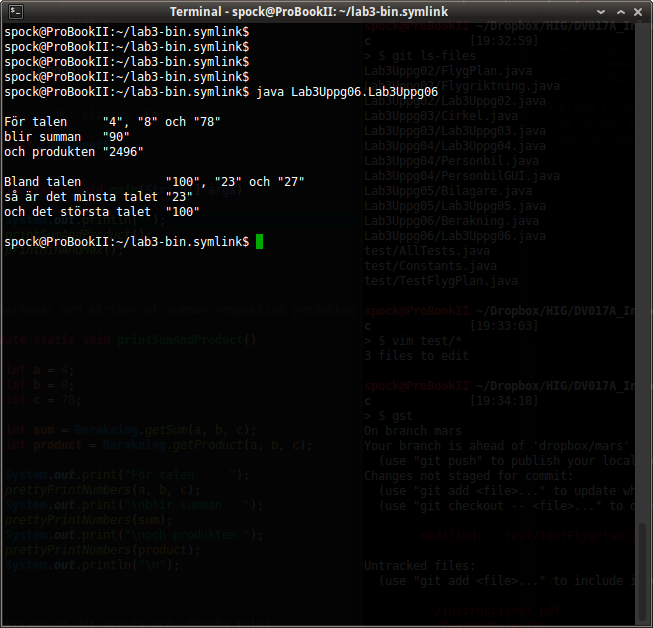
\includegraphics[width=\linewidth]{img/06.png}
    \caption{Körning av koden till Uppgift~\ref{sec:uppg06}}
    \label{fig:uppg06-screenshot}
\end{figure}

